\normaltrue \difficilefalse \tdifficilefalse
\correctionfalse
%\UPSTIidClasse{11} % 11 sup, 12 spé
%\newcommand{\UPSTIidClasse}{12}

\exer{Pompe à palettes  $\star$ \label{B2:13:PTSI:10}}
\setcounter{question}{0}\UPSTIcompetence[2]{B2-13}
\index{Compétence B2-13-PTSI}
\index{Pompe à palettes}
\ifcorrection
\else
\marginnote{\textbf{Pas de corrigé pour cet exercice.}}
\fi

\ifprof
\else
Soit le mécanisme suivant.
\begin{center}
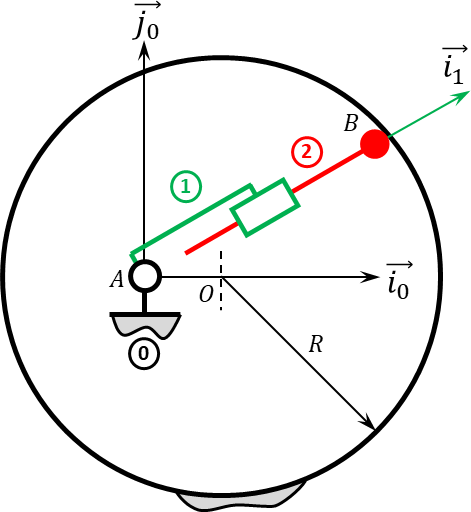
\includegraphics[width=.65\linewidth]{10_01}
\end{center}

\fi


\question{Réaliser le paramétrage du mécanisme.}

\ifprof

\else
\fi


\ifprof
\else
\footnotesize
\ifcolle
\else

\fi

\normalsize
\begin{flushright}
\footnotesize{Corrigé  voir \ref{B2:13:PTSI:10}.}
\end{flushright}%
\fi